\documentclass[border=10mm]{standalone}

\usepackage[margin=1in]{geometry}
\usepackage{graphicx}
\usepackage{bm}
\usepackage{pgfplots}
\usepackage{tikz}
\usetikzlibrary{calc}
\def\MarkRightAngle[size=#1](#2,#3,#4){
  \draw[] ($(#3)!#1!(#2)$) -- ($($(#3)!#1!(#2)$)!#1!90:(#2)$) -- ($(#3)!#1!(#4)$)
}

\usetikzlibrary{patterns}
\usetikzlibrary{angles,quotes}
\usepackage{parskip}
\usetikzlibrary{intersections, pgfplots.fillbetween}
\usepackage{amsmath}
\usepackage{multicol}
\usepackage{enumitem}
\usepackage{multirow}


\begin{document}


\tikzset{every picture/.style={line width=0.75pt}} % line width        

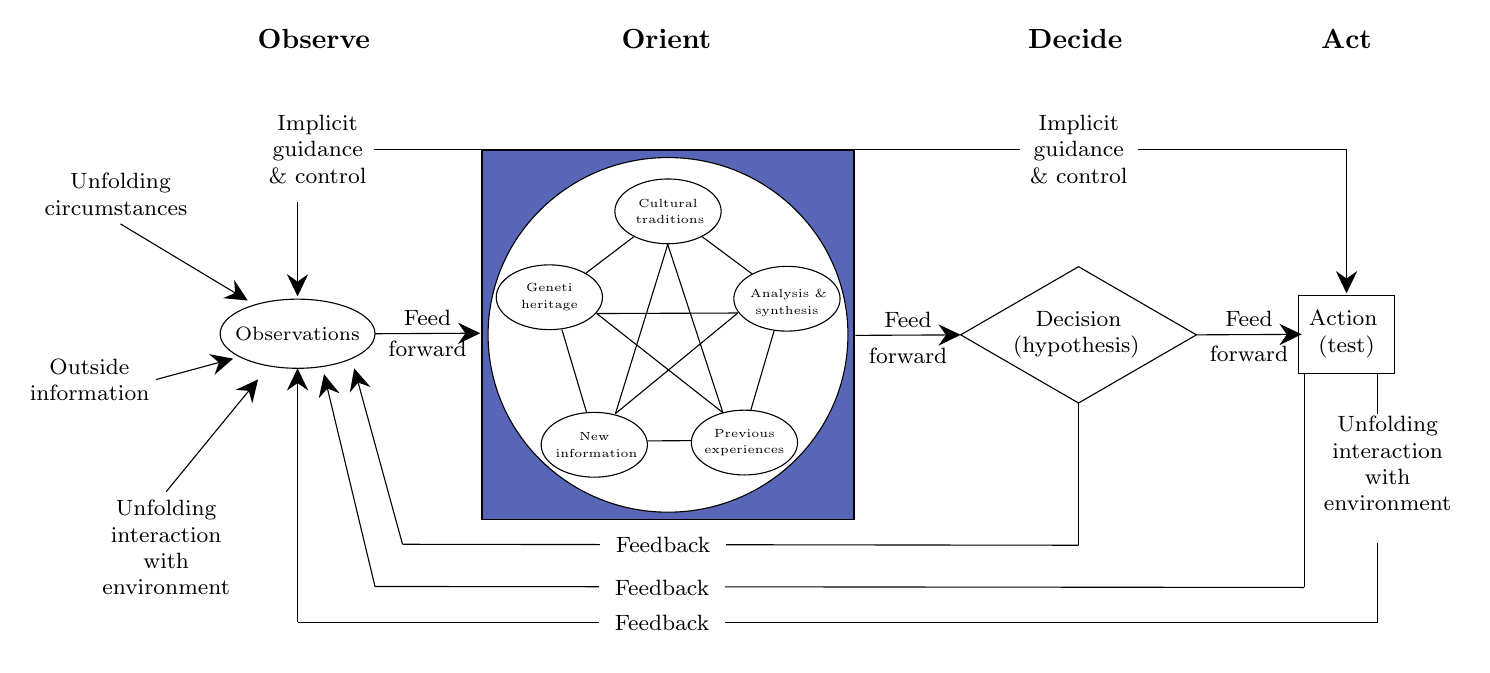
\begin{tikzpicture}[x=0.75pt,y=0.75pt,yscale=-1,xscale=1]


%Shape: Rectangle 
\draw  [fill={rgb, 255:red, 88; green, 102; blue, 184 }  ,fill opacity=1 ] (223.16,121.09) -- (402.38,121.09) -- (402.38,298.78) -- (223.16,298.78) -- cycle ;
%Shape: Ellipse 
\draw  [fill={rgb, 255:red, 255; green, 255; blue, 255 }  ,fill opacity=1 ] (226.08,209.93) .. controls (226.08,162.75) and (264.89,124.5) .. (312.77,124.5) .. controls (360.65,124.5) and (399.47,162.75) .. (399.47,209.93) .. controls (399.47,257.12) and (360.65,295.37) .. (312.77,295.37) .. controls (264.89,295.37) and (226.08,257.12) .. (226.08,209.93) -- cycle ;
%Shape: Ellipse 
\draw   (344.49,192.53) .. controls (344.49,183.91) and (355.95,176.92) .. (370.08,176.92) .. controls (384.22,176.92) and (395.68,183.91) .. (395.68,192.53) .. controls (395.68,201.15) and (384.22,208.14) .. (370.08,208.14) .. controls (355.95,208.14) and (344.49,201.15) .. (344.49,192.53) -- cycle ;
%Shape: Ellipse 
\draw   (287.18,150.43) .. controls (287.18,141.81) and (298.63,134.82) .. (312.77,134.82) .. controls (326.91,134.82) and (338.37,141.81) .. (338.37,150.43) .. controls (338.37,159.05) and (326.91,166.04) .. (312.77,166.04) .. controls (298.63,166.04) and (287.18,159.05) .. (287.18,150.43) -- cycle ;
%Shape: Ellipse  
\draw   (324.01,261.82) .. controls (324.01,253.2) and (335.47,246.21) .. (349.61,246.21) .. controls (363.74,246.21) and (375.2,253.2) .. (375.2,261.82) .. controls (375.2,270.44) and (363.74,277.43) .. (349.61,277.43) .. controls (335.47,277.43) and (324.01,270.44) .. (324.01,261.82) -- cycle ;
%Shape: Ellipse 
\draw   (251.66,262.89) .. controls (251.66,254.27) and (263.12,247.28) .. (277.26,247.28) .. controls (291.39,247.28) and (302.85,254.27) .. (302.85,262.89) .. controls (302.85,271.52) and (291.39,278.51) .. (277.26,278.51) .. controls (263.12,278.51) and (251.66,271.52) .. (251.66,262.89) -- cycle ;
%Shape: Ellipse  
\draw   (230.02,191.82) .. controls (230.02,183.2) and (241.48,176.21) .. (255.62,176.21) .. controls (269.75,176.21) and (281.21,183.2) .. (281.21,191.82) .. controls (281.21,200.44) and (269.75,207.43) .. (255.62,207.43) .. controls (241.48,207.43) and (230.02,200.44) .. (230.02,191.82) -- cycle ;
%Straight Lines 
\draw    (346.4,199.41) -- (287.46,247.88) ;
%Straight Lines 
\draw    (312.77,166.76) -- (339.21,247.41) ;
%Straight Lines  
\draw    (312.77,166.04) -- (287.46,247.88) ;
%Straight Lines 
\draw    (278.42,199.66) -- (339.21,247.41) ;
%Straight Lines 
\draw    (346.4,199.41) -- (278.42,199.66) ;
%Straight Lines 
\draw    (261.67,207.43) -- (273.5,247.16) ;
%Straight Lines 
\draw    (296.24,162.7) -- (273.2,180.22) ;
%Straight Lines  
\draw    (353.26,180.53) -- (329.3,162.7) ;
%Straight Lines 
\draw    (352.65,246.22) -- (363.87,208.06) ;
%Straight Lines 
\draw    (324.11,260.89) -- (302.85,261.02) ;
%Straight Lines 
\draw    (171.15,120.46) -- (639.69,120.46) ;
%Shape: Ellipse 
\draw   (97,209.39) .. controls (97,200.19) and (113.7,192.73) .. (134.3,192.73) .. controls (154.9,192.73) and (171.6,200.19) .. (171.6,209.39) .. controls (171.6,218.59) and (154.9,226.05) .. (134.3,226.05) .. controls (113.7,226.05) and (97,218.59) .. (97,209.39) -- cycle ;

%Straight Lines 
\draw    (219.3,209.15) -- (171.6,209.39) ;
\draw [shift={(222.3,209.14)}, rotate = 179.72] [fill={rgb, 255:red, 0; green, 0; blue, 0 }  ][line width=0.08]  [draw opacity=0] (10.72,-5.15) -- (0,0) -- (10.72,5.15) -- (7.12,0) -- cycle    ;
%Straight Lines 
\draw    (450.79,209.95) -- (403.09,210.18) ;
\draw [shift={(453.79,209.93)}, rotate = 179.72] [fill={rgb, 255:red, 0; green, 0; blue, 0 }  ][line width=0.08]  [draw opacity=0] (10.72,-5.15) -- (0,0) -- (10.72,5.15) -- (7.12,0) -- cycle    ;
%Shape: Diamond 
\draw   (510.57,177.09) -- (567.36,209.93) -- (510.57,242.78) -- (453.79,209.93) -- cycle ;
%Straight Lines 
\draw    (615.05,209.7) -- (567.36,209.93) ;
\draw [shift={(618.05,209.69)}, rotate = 179.72] [fill={rgb, 255:red, 0; green, 0; blue, 0 }  ][line width=0.08]  [draw opacity=0] (10.72,-5.15) -- (0,0) -- (10.72,5.15) -- (7.12,0) -- cycle    ;
%Shape: Rectangle  
\draw   (616.49,190.85) -- (662.89,190.85) -- (662.89,228.39) -- (616.49,228.39) -- cycle ;
%Straight Lines 
\draw    (639.69,120.46) -- (639.69,186.91) ;
\draw [shift={(639.69,189.91)}, rotate = 270] [fill={rgb, 255:red, 0; green, 0; blue, 0 }  ][line width=0.08]  [draw opacity=0] (10.72,-5.15) -- (0,0) -- (10.72,5.15) -- (7.12,0) -- cycle    ;
%Straight Lines  
\draw    (654.7,228.39) -- (654.7,248.1) ;
%Straight Lines  
\draw    (654.7,310.04) -- (654.7,348.52) ;
%Straight Lines 
\draw    (619.22,228.39) -- (619.22,331.63) ;
%Straight Lines 
\draw    (134.3,348.52) -- (654.7,348.52) ;
%Straight Lines  
\draw    (134.3,229.05) -- (134.3,348.05) ;
\draw [shift={(134.3,226.05)}, rotate = 90] [fill={rgb, 255:red, 0; green, 0; blue, 0 }  ][line width=0.08]  [draw opacity=0] (10.72,-5.15) -- (0,0) -- (10.72,5.15) -- (7.12,0) -- cycle    ;
%Straight Lines  
\draw    (171.6,331.16) -- (619.22,331.63) ;
%Straight Lines 
\draw    (510.57,242.78) -- (510.57,311.29) ;
%Straight Lines 
\draw    (184.87,310.83) -- (510.57,311.29) ;
%Straight Lines  
\draw    (162.39,228.94) -- (184.87,310.83) ;
\draw [shift={(161.59,226.05)}, rotate = 74.65] [fill={rgb, 255:red, 0; green, 0; blue, 0 }  ][line width=0.08]  [draw opacity=0] (10.72,-5.15) -- (0,0) -- (10.72,5.15) -- (7.12,0) -- cycle    ;
%Straight Lines  
\draw    (147.74,231.78) -- (171.6,331.16) ;
\draw [shift={(147.04,228.86)}, rotate = 76.5] [fill={rgb, 255:red, 0; green, 0; blue, 0 }  ][line width=0.08]  [draw opacity=0] (10.72,-5.15) -- (0,0) -- (10.72,5.15) -- (7.12,0) -- cycle    ;
%Straight Lines 
\draw    (134.3,145.94) -- (134.3,188.39) ;
\draw [shift={(134.3,191.39)}, rotate = 270] [fill={rgb, 255:red, 0; green, 0; blue, 0 }  ][line width=0.08]  [draw opacity=0] (10.72,-5.15) -- (0,0) -- (10.72,5.15) -- (7.12,0) -- cycle    ;
%Straight Lines 
\draw    (49,156.5) -- (107.73,191.84) ;
\draw [shift={(110.3,193.39)}, rotate = 211.04] [fill={rgb, 255:red, 0; green, 0; blue, 0 }  ][line width=0.08]  [draw opacity=0] (10.72,-5.15) -- (0,0) -- (10.72,5.15) -- (7.12,0) -- cycle    ;
%Straight Lines  
\draw    (66,231.5) -- (100.41,222.17) ;
\draw [shift={(103.3,221.39)}, rotate = 164.83] [fill={rgb, 255:red, 0; green, 0; blue, 0 }  ][line width=0.08]  [draw opacity=0] (10.72,-5.15) -- (0,0) -- (10.72,5.15) -- (7.12,0) -- cycle    ;
%Straight Lines  
\draw    (71,285.5) -- (113.4,233.71) ;
\draw [shift={(115.3,231.39)}, rotate = 129.31] [fill={rgb, 255:red, 0; green, 0; blue, 0 }  ][line width=0.08]  [draw opacity=0] (10.72,-5.15) -- (0,0) -- (10.72,5.15) -- (7.12,0) -- cycle    ;

% Text Node
\draw (255.62,191.82) node  [font=\tiny] [align=left] {\begin{minipage}[lt]{21.15pt}\setlength\topsep{0pt}
\begin{center}
\scalebox{.85}{Geneti}\\\scalebox{.85}{heritage}
\end{center}

\end{minipage}};
% Text Node
\draw (370.08,192.53) node  [font=\tiny] [align=left] {\begin{minipage}[lt]{26.53pt}\setlength\topsep{0pt}
\begin{center}
\scalebox{.85}{Analysis \&}\\\scalebox{.85}{synthesis}
\end{center}

\end{minipage}};
% Text Node
\draw (277.26,262.89) node  [font=\tiny] [align=left] {\begin{minipage}[lt]{27.95pt}\setlength\topsep{0pt}
\begin{center}
\scalebox{.85}{New}\\\scalebox{.85}{information}
\end{center}

\end{minipage}};
% Text Node
\draw (349.61,261.82) node  [font=\tiny] [align=left] {\begin{minipage}[lt]{30.23pt}\setlength\topsep{0pt}
\begin{center}
\scalebox{.85}{Previous}\\\scalebox{.85}{experiences}
\end{center}

\end{minipage}};
% Text Node
\draw (312.77,150.43) node  [font=\tiny] [align=left] {\begin{minipage}[lt]{23.42pt}\setlength\topsep{0pt}
\begin{center}
\scalebox{.85}{Cultural}\\\scalebox{.85}{traditions}
\end{center}

\end{minipage}};
% Text Node
\draw (142.15,73.46) node [anchor=south] [inner sep=0.75pt]   [align=left] {\textbf{Observe}};
% Text Node
\draw (312,73.46) node [anchor=south] [inner sep=0.75pt]   [align=left] {\textbf{Orient}};
% Text Node
\draw (509,73.46) node [anchor=south] [inner sep=0.75pt]   [align=left] {\textbf{Decide}};
% Text Node
\draw (639.69,73.46) node [anchor=south] [inner sep=0.75pt]   [align=left] {\textbf{Act}};
% Text Node
\draw (169.15,120.46) node [anchor=east] [inner sep=0.75pt]  [font=\footnotesize] [align=left] {\begin{minipage}[lt]{35.85pt}\setlength\topsep{0pt}
\begin{center}
Implicit\\guidance\\\& control
\end{center}

\end{minipage}};
% Text Node
\draw  [draw opacity=0][fill={rgb, 255:red, 255; green, 255; blue, 255 }  ,fill opacity=1 ]  (482.19,93.46) -- (539.19,93.46) -- (539.19,147.46) -- (482.19,147.46) -- cycle  ;
\draw (510.69,120.46) node  [font=\footnotesize] [align=left] {\begin{minipage}[lt]{35.85pt}\setlength\topsep{0pt}
\begin{center}
Implicit\\guidance\\\& control
\end{center}

\end{minipage}};
% Text Node
\draw (428.44,207.64) node [anchor=south] [inner sep=0.75pt]  [font=\footnotesize] [align=left] {Feed};
% Text Node
\draw (428.44,215.29) node [anchor=north] [inner sep=0.75pt]  [font=\footnotesize] [align=left] {forward};
% Text Node
\draw (510.57,209.93) node  [font=\footnotesize] [align=left] {\begin{minipage}[lt]{47.18pt}\setlength\topsep{0pt}
\begin{center}
Decision
\end{center}
(hypothesis)
\end{minipage}};
% Text Node
\draw (592.71,207.39) node [anchor=south] [inner sep=0.75pt]  [font=\footnotesize] [align=left] {Feed};
% Text Node
\draw (592.71,214.1) node [anchor=north] [inner sep=0.75pt]  [font=\footnotesize] [align=left] {forward};
% Text Node
\draw (639.69,209.62) node  [font=\footnotesize] [align=left] {\begin{minipage}[lt]{27.22pt}\setlength\topsep{0pt}
Action
\begin{center}
(test)
\end{center}

\end{minipage}};
% Text Node
\draw (196.95,206.85) node [anchor=south] [inner sep=0.75pt]  [font=\footnotesize] [align=left] {Feed};
% Text Node
\draw (196.95,211.68) node [anchor=north] [inner sep=0.75pt]  [font=\footnotesize] [align=left] {forward};
% Text Node
\draw (49,153.5) node [anchor=south] [inner sep=0.75pt]  [font=\footnotesize] [align=left] {\begin{minipage}[lt]{54.87pt}\setlength\topsep{0pt}
\begin{center}
Unfolding
\end{center}
circumstances
\end{minipage}};
% Text Node
\draw (64,231.5) node [anchor=east] [inner sep=0.75pt]  [font=\footnotesize] [align=left] {\begin{minipage}[lt]{43.1pt}\setlength\topsep{0pt}
\begin{center}
Outside
\end{center}
information
\end{minipage}};
% Text Node
\draw (71,288.5) node [anchor=north] [inner sep=0.75pt]  [font=\footnotesize] [align=left] {\begin{minipage}[lt]{47.63pt}\setlength\topsep{0pt}
\begin{center}
Unfolding\\interaction\\with\\environment
\end{center}

\end{minipage}};
% Text Node
\draw  [draw opacity=0][fill={rgb, 255:red, 255; green, 255; blue, 255 }  ,fill opacity=1 ]  (279.39,321.13) -- (340.39,321.13) -- (340.39,342.13) -- (279.39,342.13) -- cycle  ;
\draw (309.89,331.63) node  [font=\footnotesize] [align=left] {Feedback};
% Text Node
\draw  [draw opacity=0][fill={rgb, 255:red, 255; green, 255; blue, 255 }  ,fill opacity=1 ]  (279.39,338.02) -- (340.39,338.02) -- (340.39,359.02) -- (279.39,359.02) -- cycle  ;
\draw (309.89,348.52) node  [font=\footnotesize] [align=left] {Feedback};
% Text Node
\draw  [draw opacity=0][fill={rgb, 255:red, 255; green, 255; blue, 255 }  ,fill opacity=1 ]  (279.92,300.56) -- (340.92,300.56) -- (340.92,321.56) -- (279.92,321.56) -- cycle  ;
\draw (310.42,311.06) node  [font=\footnotesize] [align=left] {Feedback};
% Text Node
\draw (623.47,248.04) node [anchor=north west][inner sep=0.75pt]  [font=\footnotesize] [align=left] {\begin{minipage}[lt]{52.17pt}\setlength\topsep{0pt}
\begin{center}
Unfolding\\interaction\\with\\environment
\end{center}

\end{minipage}};
% Text Node
\draw (134.3,209.39) node  [font=\scriptsize] [align=left] {Observations};


\end{tikzpicture}


% This version of John Boyd's OODA Loop appeared in Hoofnagle & Richard's Cybersecurity in Context (Wiley 2024) and is adapted to Latex by Malik @hadimalik1 on Fiverr
\end{document}

